% Options for packages loaded elsewhere
\PassOptionsToPackage{unicode}{hyperref}
\PassOptionsToPackage{hyphens}{url}
%
\documentclass[
]{article}
\usepackage{amsmath,amssymb}
\usepackage{lmodern}
\usepackage{iftex}
\ifPDFTeX
  \usepackage[T1]{fontenc}
  \usepackage[utf8]{inputenc}
  \usepackage{textcomp} % provide euro and other symbols
\else % if luatex or xetex
  \usepackage{unicode-math}
  \defaultfontfeatures{Scale=MatchLowercase}
  \defaultfontfeatures[\rmfamily]{Ligatures=TeX,Scale=1}
\fi
% Use upquote if available, for straight quotes in verbatim environments
\IfFileExists{upquote.sty}{\usepackage{upquote}}{}
\IfFileExists{microtype.sty}{% use microtype if available
  \usepackage[]{microtype}
  \UseMicrotypeSet[protrusion]{basicmath} % disable protrusion for tt fonts
}{}
\makeatletter
\@ifundefined{KOMAClassName}{% if non-KOMA class
  \IfFileExists{parskip.sty}{%
    \usepackage{parskip}
  }{% else
    \setlength{\parindent}{0pt}
    \setlength{\parskip}{6pt plus 2pt minus 1pt}}
}{% if KOMA class
  \KOMAoptions{parskip=half}}
\makeatother
\usepackage{xcolor}
\usepackage[margin=1in]{geometry}
\usepackage{longtable,booktabs,array}
\usepackage{calc} % for calculating minipage widths
% Correct order of tables after \paragraph or \subparagraph
\usepackage{etoolbox}
\makeatletter
\patchcmd\longtable{\par}{\if@noskipsec\mbox{}\fi\par}{}{}
\makeatother
% Allow footnotes in longtable head/foot
\IfFileExists{footnotehyper.sty}{\usepackage{footnotehyper}}{\usepackage{footnote}}
\makesavenoteenv{longtable}
\usepackage{graphicx}
\makeatletter
\def\maxwidth{\ifdim\Gin@nat@width>\linewidth\linewidth\else\Gin@nat@width\fi}
\def\maxheight{\ifdim\Gin@nat@height>\textheight\textheight\else\Gin@nat@height\fi}
\makeatother
% Scale images if necessary, so that they will not overflow the page
% margins by default, and it is still possible to overwrite the defaults
% using explicit options in \includegraphics[width, height, ...]{}
\setkeys{Gin}{width=\maxwidth,height=\maxheight,keepaspectratio}
% Set default figure placement to htbp
\makeatletter
\def\fps@figure{htbp}
\makeatother
\setlength{\emergencystretch}{3em} % prevent overfull lines
\providecommand{\tightlist}{%
  \setlength{\itemsep}{0pt}\setlength{\parskip}{0pt}}
\setcounter{secnumdepth}{5}
\newlength{\cslhangindent}
\setlength{\cslhangindent}{1.5em}
\newlength{\csllabelwidth}
\setlength{\csllabelwidth}{3em}
\newlength{\cslentryspacingunit} % times entry-spacing
\setlength{\cslentryspacingunit}{\parskip}
\newenvironment{CSLReferences}[2] % #1 hanging-ident, #2 entry spacing
 {% don't indent paragraphs
  \setlength{\parindent}{0pt}
  % turn on hanging indent if param 1 is 1
  \ifodd #1
  \let\oldpar\par
  \def\par{\hangindent=\cslhangindent\oldpar}
  \fi
  % set entry spacing
  \setlength{\parskip}{#2\cslentryspacingunit}
 }%
 {}
\usepackage{calc}
\newcommand{\CSLBlock}[1]{#1\hfill\break}
\newcommand{\CSLLeftMargin}[1]{\parbox[t]{\csllabelwidth}{#1}}
\newcommand{\CSLRightInline}[1]{\parbox[t]{\linewidth - \csllabelwidth}{#1}\break}
\newcommand{\CSLIndent}[1]{\hspace{\cslhangindent}#1}
\usepackage{amstext}
\usepackage{amsmath}
\usepackage{booktabs}
\usepackage{longtable}
\usepackage{array}
\usepackage{multirow}
\usepackage{wrapfig}
\usepackage{float}
\usepackage{colortbl}
\usepackage{pdflscape}
\usepackage{tabu}
\usepackage{threeparttable}
\usepackage{threeparttablex}
\usepackage[normalem]{ulem}
\usepackage{makecell}
\usepackage{xcolor}
\usepackage{algorithm,algorithmic}
\AtBeginEnvironment{CSLReferences}{\small}
\usepackage{tabularx}
\ifLuaTeX
  \usepackage{selnolig}  % disable illegal ligatures
\fi
\IfFileExists{bookmark.sty}{\usepackage{bookmark}}{\usepackage{hyperref}}
\IfFileExists{xurl.sty}{\usepackage{xurl}}{} % add URL line breaks if available
\urlstyle{same} % disable monospaced font for URLs
\hypersetup{
  pdftitle={Directed topic extraction with side information for sustainability analysis},
  pdfauthor={Maria Osipenko},
  hidelinks,
  pdfcreator={LaTeX via pandoc}}

\title{Directed topic extraction with side information for sustainability analysis}
\author{Maria Osipenko}
\date{2024-02-19}

\begin{document}
\maketitle

\hypertarget{abstract}{%
\section{Abstract}\label{abstract}}

Topic analysis represents each document of a text corpus in a low dimensional latent topic space. In some cases the desired topic representation is prestructured in form of requirements or guidelines delivering side information. For instance, investors can be interested in automatically assessing sustainability in textual content of corporate reports with a focus on the established 17 UN sustainability goals. The main corpus here contains the corporate report texts, and the texts with the definitions of the 17 UN sustainability goals represent the side information. Under assumption that both text corpora share a common low dimensional subspace, we propose to represent them in a such via directed topic extraction by matrix co-factorization. Both, the main and the side text corpora are first represented as term-document matrices, which are then jointly decomposed into word-topic and topic-document matrices. Thereby, the word-topic matrix is common to both text corpora, whereas the topic-document matrices contain specific representations in the shared topic space. A nuisance parameter, which allows to move focus between error minimization of individual factorization terms, controls the extent, to which the side information is taken into account. With our approach, documents from the main and the side corpora can be related to each other in the resulting latent topic space. That is, the considered corporate reports are represented in the same latent topic space as the descriptions of the 17 UN sustainability goals, such that a structured automatic sustainability assessment of textual reports content is possible. We provide an algorithm for such directed topic extraction and propose techniques for visualizing and interpreting the results.

\hypertarget{introduction}{%
\section{Introduction}\label{introduction}}

The market for sustainable investments grows steadily. However, there are no uniform standards for comparing/quantifying sustainability levels of firms. Although several agencies provide in the mean time environmental, social, governance (ESG) rating, Berg, Kölbel, and Rigobon (2022) points out the disagreement of such ratings across the rating agencies. In this situation, it seems hard to overview the ESG development of potential investment firms and decide upon investors ESG value system.

Kang and Kim (2022) proposes to take into account other textual sources of information on sustainability easily available to private investors:

\begin{itemize}
\item
  corporate responsibility reports
\item
  sustainability reports
\item
  environmental action reports
\end{itemize}

or similar freely available sustainability related reports. Kang and Kim (2022) propose to process these unstructured information sources with regard to an established systematic - commonly accepted 17 UN sustainable development goals (SDGs, \url{https://sdgs.un.org/goals}). SDGs represent intergovernmental set of 17 goals which broadly address modern environmental and social challenges adopted in 2015 by the UN General Assembly. The goal is to structure the information from textual sustainability reports with the respect to the SDGs in a way, which enables a sound comparison of companies' contribution to solving those major challenges. The authors in Kang and Kim (2022) employ sentence similarity method to assess the relatedness of the reports to the goals. However, their approach ignores semantic relations between words, which may have similar meaning. To overcome the limitation in this paper, we propose a co-matrix factorization methodology to leverage information from the textual sources via automatic topic extraction while considering the value system established by the 17 SDGs.

Topic analysis (Churchill and Singh (2022)) represents each document in a collection of documents in a low dimensional latent topic space. The most popular classical methods are Latent (probabilistic) semantic analysis (Deerwester et al. (1990), Hofmann (1999)), Latent dirichlet allocation (LDA, Blei, Ng, and Jordan (2003)) as well as general purpose dimension reduction methods as non-negative matrix factorization (NMF, Lee and Seung (2000), Vangara et al. (2020)), and extensions of the methods above (e.g.~in Yang and Li (2015/07), Suleman and Korkontzelos (2021), and Figuera and García Bringas (2024)). Recently, also deep neural network based models have been proposed (Zhao et al. (2021)).

Topic extraction for structuring text data has been used extensively used in financial literature. For instance, Li et al. (2017) employ Latent Dirichlet Allocation (LDA) to structure financial stability reports. Yu Chen et al. (2017) compares Principal component analysis, NMF, LDA and deep learning models for text analytics in banking. W. Chen et al. (2023) uses LDA and neural network based models to analyse news impact on financial markets. For a comprehensive review of text mining and topic analysis in finance literature, we refer to LOUGHRAN and MCDONALD (2016) and Gupta et al. (2020). Despite the popularity of LDA, Yong Chen et al. (2019) and Egger and Yu (2022) argue, that NMF can outperform the latter by extracting interpretable topics, especially for short texts. Since we are going to cut the reports into small peaces of context, NMF is a promising technique for our needs. Moreover, Nugumanova et al. (2022) highlights the advantage of NMF-based methods for efficient extraction of domain specific terms, which is also relevant for our task with sustainability focus.

Recently, several LDA-based topic extraction methods that allow to explicitly embed known structure or side information have been proposed. For instance, Harandizadeh, Priniski, and Morstatter (2022) proposes to use word2vec embeddings combined with LDA and vocabulary priors to obtain interpretable word embeddings. Eshima, Imai, and Sasaki (2023) embed prespecified keywords in LDA for the same reason. In the same spirit, Watanabe and Zhou (2022) use seeded LDA with a carefuly chosen seeded vocabulary to assist in classifying documents in specific categories. With their approaches, the authors account for additional information in topic extraction. The draw back of the mentioned approaches in Watanabe and Zhou (2022) and Eshima, Imai, and Sasaki (2023) lies in the need of manual intervention for keyword or vocabulary specification. Harandizadeh, Priniski, and Morstatter (2022) uses word vectors from a pretrained general purpose word2vec model and thus, it is not clear, whether their model works for specific domains as sustainability reports.

On the other hand, there exist matrix factorization based approaches which integrate side information into dimension reduction. Rao et al. (2015) and later Zhang et al. (2020) propose to integrate side information using graphs. They derive a graph regularized version of matrix factorization and an associated alternating algorithm. However, their side information is not high dimensional and incorporates few individual characteristics which build basis for the graph links. Yet another way to consider high dimensional additional information are matrix co-factorization techniques.
Co-factorization techniques factorize two or three matrices with some common cofactors simultaneously. For instance, Fang and Si (2011) consider user communities information and Luo et al. (2019) incorporate tagging and time stamp of ratings in their personalized recommendations via matrix co-factorization. The approach is transparent and easily adjustable. By introducing a nuisance parameter which allows to move the focus between error minimization of individual factorization terms, additional flexibility is ensured.

In this paper, we propose a topic model based on non-negative matrix co-factorazition (NMCF) to extract sustainability related topics from the related textual sources with the 17 UN goals as side information. The advantages of our approach include a fully automated topic extraction (without manual key word search), its interpretability, adaptivity (via nuisance parameter \(\lambda\)), and simple implementation.

The paper is structured as follows. In the next chapter, we explain the method used and derive the NMCF algorithm for topic extraction with side information. We also introduce the data in form of sustainability related reporting and the 17 UN goals, and describe our preprocessing steps. The results of the application of our algorithm to the data follow. Finally, we conclude and discuss future research directions.

\hypertarget{methods-and-data}{%
\section{Methods and Data}\label{methods-and-data}}

In this section, we explain the method used and derive the NMCF algorithm for topic extraction with side information. Subsequently, we introduce the data in form of sustainability related reporting and the 17 UN goals, and describe our preprocessing steps.

\hypertarget{matrix-co-factorization-for-sustainability-analysis}{%
\subsection{Matrix co-factorization for sustainability analysis}\label{matrix-co-factorization-for-sustainability-analysis}}

We assume that the corporate reports texts share a common topic structure with the sustainability goals definition but also contain some other topics concerning e.g.~financial statements. Moreover, we anticipate that the goals are written very focused using concrete sparse vocabulary, whereas the reports may refer to the same concepts using other wordings. That is, a common topic may contain words that are semantically relevant to sustainability goals vocabulary but not directly mentioned in the texts of the SDGs.
That is, we assume, that both text corpora share a common low dimensional subspace, in which they can be compared to each other by means of some distance measure.

To account for the mentioned issues, we define the following model for terms-document matrices arising from reports and sustainability goals texts.

\[M = U^\top V + E\]

and

\[C = U^\top Q + F\]

where

\begin{itemize}
\tightlist
\item
  \(M\) is the (weighted) term-context matrix for the corporate reports with dimensions \((p\times n)\), where \(p\) is the joint vocabulary (words and phrases with two co-occurring words) obtained from both reports and sustainability goals texts. \(n\) is the number of corporate reports contexts, where the later represents one page of a corporate report. The overall dimensions for \(M\) for our data are \((18'086\times 6'891)\).
\item
  \(C\) is the (weighted) term-context matrix for the sustainability goals with dimensions \((p\times m)\), where \(p\) is again the joint vocabulary (words and phrases with two co-occurring words) obtained from both reports and sustainability goals texts. \(m\) is the number of sustainability goals contexts, where each context represents each of the \(17\) goals. The overall dimensions for \(C\) for our data are \((18'086\times 17)\).
\item
  \(U\) is the term-topic representation matrix of dimensions \((p\times k+\tilde k)\), where \(k\) is the number of common topics and \(\tilde k\) is the number of topics.
\item
  \(V\) is the context-topic representation matrix for the reports of dimensions \((k+\tilde k\times n)\).
\item
  \(Q\) is the context-topic representation matrix for sustainability goals of dimensions \((k\times m)\).
\item
  \(E\) and \(F\) are matrices of error terms of dimensions \((p\times n)\) and \((p\times m)\) respectively.
\end{itemize}

The associated topic extraction problem is then:

\begin{equation}\min(||M - U^\top V||^2 + \lambda ||C-U_0^\top Q||^2)\label{eq:minc}
\end{equation}

where \(\lambda\) adapts the importance of the loss on the second factorization term (see Figure for a schematic representation of the approach).

\hfil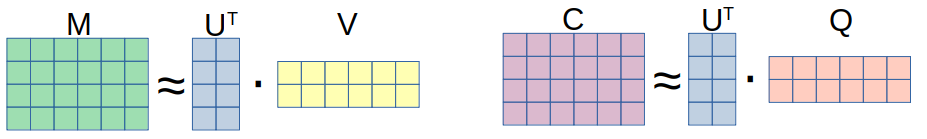
\includegraphics[width=1\textwidth,height=\textheight]{./images/mf2.png}\hfil

The value of \(\lambda\) balances out the combined loss function. It is responsible for adjusting the impact of accuracy concerning reports versus SDGs. Since the second dimension of \(C\) is much lower than that of \(M\), the first part of the loss will dominate the co-factorization. To give more weight to the second part one can alternate \(\lambda\).

Because of the non-negativity of the entries in \(M\) and \(C\) it makes sense to restrict at least \(U\) to be non-negative. This enhances the interpretability and sparsity of the resulting topics \textbf{(see cite)}. So the minimization is subject to:

\begin{equation}U, V,Q \geq 0 \text{ elementwise.}\label{eq:cons}
\end{equation}

The corresponding algorithm for minimizing \eqref{eq:minc} under the constraint \eqref{eq:cons} is based on the alternating minimization/ alternating projection in from of the hierarchical non-negative alternating least squares (HALS) of Cichocki, Zdunek, and Amari (2007) with our modification for the co-factorization setup (see also Degleris et al. (2019)).

For the loss function \(J(U,V,Q)\), we have:

\begin{align*}J(U,V,Q) &= ||M-U^\top V||^2 + \lambda ||C-U^\top Q|| \\
&= ||M-\sum_{k=1}^K u_kv_k^\top||^2 + \lambda ||C-\sum_{k=1}^K u_kq_k^\top||\\
&=||M-\sum_{k\not=p} u_kv_k^\top - u_pv_p^\top||^2 + \lambda ||C-\sum_{k\not=p} u_kq_k^\top - u_pq_p^\top||\\
&= Tr((M-\sum_{k\not=p} u_kv_k^\top)^\top (M-\sum_{k\not=p} u_kv_k^\top) - 2(M-\sum_{k\not=p} u_kv_k^\top)u_pv_p^\top + u_pv_p^\top v_p u_p) + \\
&+\lambda Tr((C-\sum_{k\not=p} u_kq_k^\top)^\top (C-\sum_{k\not=p} u_kq_k^\top) - 2(C-\sum_{k\not=p} u_kq_k^\top)u_pq_p^\top + u_pq_p^\top q_p u_p).
\end{align*}

The derivative with respect to \(u_p\) is:

\[\frac{\partial J(U,V,Q)}{\partial u_p} = - 2(M-\sum_{k\not=p} u_kv_k^\top)v_p^\top + 2u_pv_p^\top v_p - 2\lambda (C-\sum_{k\not=p} u_kq_k^\top)q_p^\top + 2\lambda u_pq_p^\top q_p.\]

Hence with Karush-Kuhn-Tucker conditions for optimality:

\[u_p = \max\left(0, \frac{(M-\sum_{k\not=p} u_kv_k^\top)v_p^\top + \lambda (C-\sum_{k\not=p} u_kq_k^\top)q_p^\top)}{v_p^\top v_p + \lambda q_p^\top q_p}\right).\]

The update rules for \(v_p\) and \(q_p\) do not differ from the HALS algorithm for NMF in Cichocki, Zdunek, and Amari (2007), that is:

\[v_p = \max\left(0, \frac{u_p(M-\sum_{k\not=p} u_kv_k^\top)}{u_p^\top u_p}\right),\]

\[q_p = \max\left(0, \frac{u_p(C-\sum_{k\not=p} u_kq_k^\top)}{u_p^\top u_p}\right).\]

The resulting Algorithm 1 is presented below.

\begin{algorithm}[H]
\begin{algorithmic}
\REQUIRE $K, \lambda$
\WHILE{not converged}
\FOR{$k=1$ to $K$}
\STATE update $V_k\leftarrow \max\left(\frac{U_k(M-U_{-k}^\top V_{-k})}{U_kU_k^\top },0\right)$
\STATE update $Q_k\leftarrow \max\left(\frac{U_k(C-U_{-k}^\top Q_{-k})}{U_kU_k^\top},0\right)$
\STATE update $U_k^\top \leftarrow \max\left(\frac{(M-U_{-k}^\top V_{-k})V_k^\top + \lambda (C-U_{-k}^\top Q_{-k})Q_k^\top}{ V_k^\top V_k  + \lambda Q_k^\top Q_k },0\right)$
\ENDFOR
\ENDWHILE
\end{algorithmic}
\caption{HALS algorithm for NMCF}
\end{algorithm}

\(X_k\) denotes the \(k\)th row of the matrix \(X\) and \(X_{-k}\) denotes the matrix without its \(k\)th row.

In summary, for a given \(K\) and \(\lambda\), the algorithm delivers a common low dimensional representation of \(M\) and \(C\) optimal in the sense of minimizing \(J(U,V,Q)\) under the non-negativity condition. \(U\) represents thereby a common latent topic space and \(V,Q\) are the low dimensional embeddings for the respective contexts in the topic space. The resulting low dimensional representation of corporate reports together with SDGs create a basis for choosing, evaluating and monitoring investments with respect to their impact on society and the environment.

\hypertarget{data}{%
\subsection{Data}\label{data}}

We use corporate responsibility/sustainability reports of seven listed tech companies with tickers AAPL, AMZ, DELL, GOOG, IBM, INTC, MSFT, and SSU. The associated time period includes the years 2013 (or later) to 2022 depending on availability. Our side information are the texts of the 17 UN SDGs.

We, first, structure our data in form of bag-of-words (with two-grams as terms) and construct the term-context representations with the pooled vocabulary on this basis.

All calculation are done in R (R Core Team (2023)). For the preprocessing on word level, we use R-Package Quanteda (Benoit et al. (2018)) to set up a corpus, to split in tokens, and compute the relative frequencies.

In the next step, we combine the term in a common dictionary, such that our bag-of-words representation contains all relevant terms,

\begin{verbatim}
## [1] "Number of docs is 35"
\end{verbatim}

\hypertarget{application-of-nmcf}{%
\section{Application of NMCF}\label{application-of-nmcf}}

In this section, we apply the proposed algorithm to the bag-of-words representations of reports sections and SDG texts. We propose a data-driven procedure for the choice of \(K\) and \(\lambda\), present and visualize the resulting representations, and demonstrate their usefulness for sustainability assessment.

\hypertarget{choosing-lambda-and-k}{%
\subsection{\texorpdfstring{Choosing \(\lambda\) and \(K\)}{Choosing \textbackslash lambda and K}}\label{choosing-lambda-and-k}}

In order to accomplish the NMCF via the Algorithm 1, we have to specify our choice of the number of topics \(K\) (which corresponds to the dimension of the latent topic space) and the nuisance parameter \(\lambda\) of the loss function. We use a data-driven procedure to simultaneously choose \(K\) and \(\lambda\) among plausible values based on maximizing the average mean-logratio topic coherence (Thompson and Mimno (2018), Selivanov, Bickel, and Wang (2022)).

We construct \(K-\lambda\) combinations with \(K=5,\ldots,15\) and \(\lambda\in[0,700],\) apply the NMCF algorithm to the described data, compute the mean-logratio coherence for each topic, and average the coherence measures subsequently over all topics.

\begin{figure}
\centering
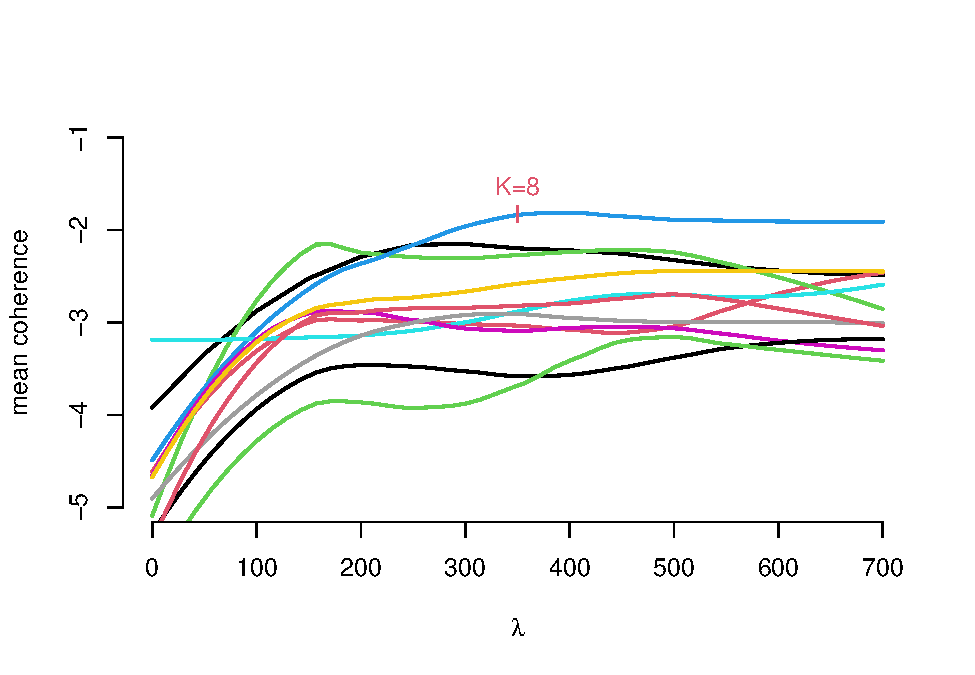
\includegraphics{20210219_sustain_dim_files/figure-latex/figtraj-1.pdf}
\caption{\label{fig:figtraj}The trajectories for the average coherence for different choices of \(K=5,6,\ldots,15\) and \(\lambda\in [0,700]\).}
\end{figure}

The resulting trajectories for diefferent \(K\) and \(\lambda\) are shown in Figure @ref\{fig:figtraj\}. The optimal number of topics is therefore \(K=8\) with \(\lambda=350.\)

\hypertarget{results}{%
\subsection{Results}\label{results}}

The result of applying Algorithm 1 are the decomposition matrices \(V,U\) and \(Q\). By looking at the largest entries of \(U\) and the corresponding terms, we can interpret the resulting latent topics. The entries of \(V,Q\) and their relative magnitudes reveal the proportions (or the importance) of the topics in the text corpus.

\begin{verbatim}
## Lade nötiges Paket: RColorBrewer
\end{verbatim}

\begin{figure}
\centering
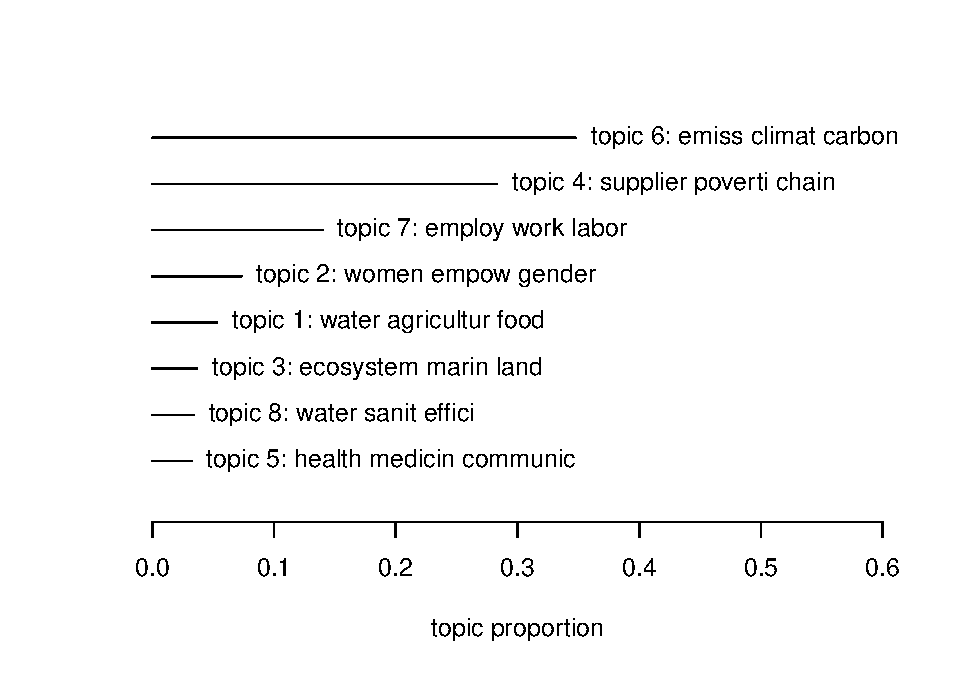
\includegraphics{20210219_sustain_dim_files/figure-latex/figtpropr-1.pdf}
\caption{\label{fig:figtpropr}Topic proportion and the words with the highest weight per topic for each of the discovered topics in the reports texts.}
\end{figure}

\begin{figure}
\centering
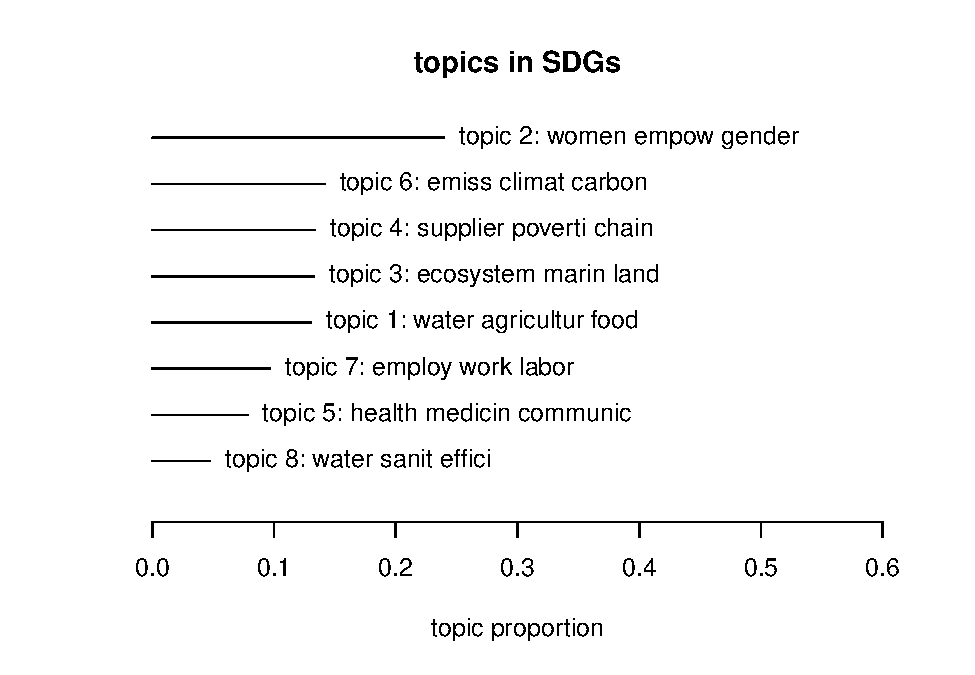
\includegraphics{20210219_sustain_dim_files/figure-latex/figtpropg-1.pdf}
\caption{\label{fig:figtpropg}Topic proportion and the words with the highest weight per topic for each of the discovered topics in the SDG texts.}
\end{figure}

Figures \ref{fig:figtpropr} and \ref{fig:figtpropg} show the topic proportions and the words with the highest weight per topic for each of the discovered topics in the reports texts and the SGD texts respectively. The top three words shown already allow to interpret the topics. The distribution of the topics is somewhat different in the report texts compared to the SDG texts. The topics ``emiss climate carbon'' and ``supplier poverti chain'' become a large share in the distribution in both reports and SDGs. Whereas the topic ``women empow gender'' seem to dominate the SDGs, it gains relatively low importance in the reports. By using this kind of representation new action areas for the companies can be discovered.

In the next figure below, we also show some chosen SDGs and the proportion of the respective topics contained in the SDG texts. The example SDGs are largely explained by the top three topics.

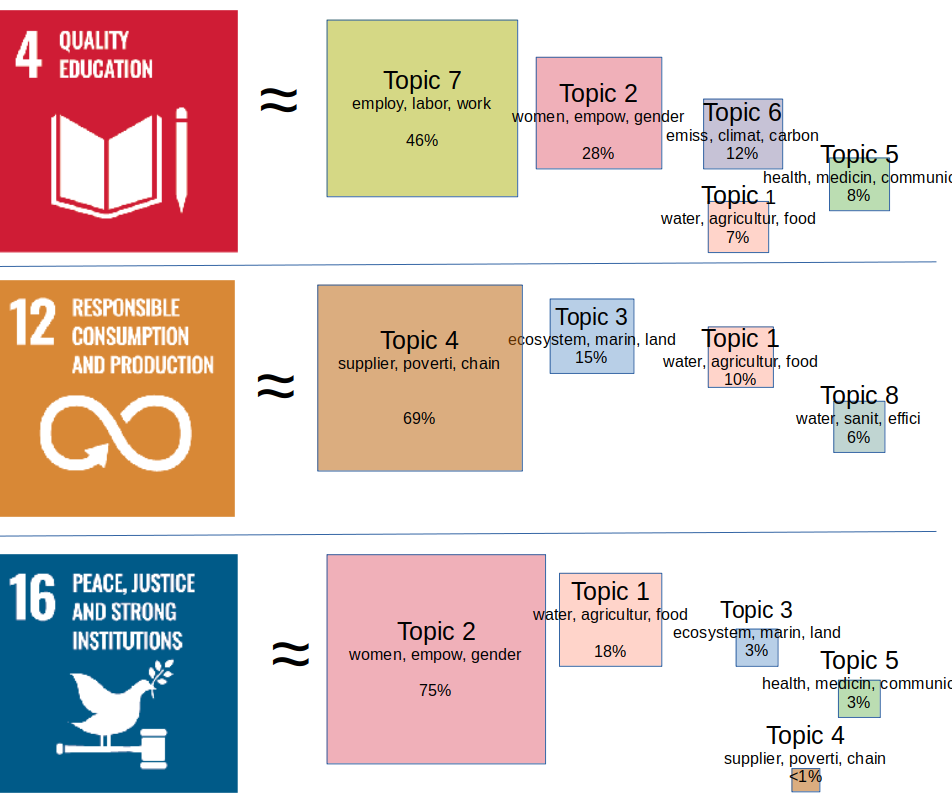
\includegraphics[width=0.9\textwidth,height=\textheight]{./images/goals_approx3.png}

Using the obtained representations of corporate reports together with SDGs we present a couple of strategies for choosing, evaluating and monitoring investments with respect to their impact on society and the environment in the following section.

\hypertarget{comparison-of-the-reports-with-goals}{%
\subsection{Comparison of the reports with goals}\label{comparison-of-the-reports-with-goals}}

Now we can use diverse (dis)similarity measures to assess the proximity of the report to the SDGs.

\begin{figure}
\centering
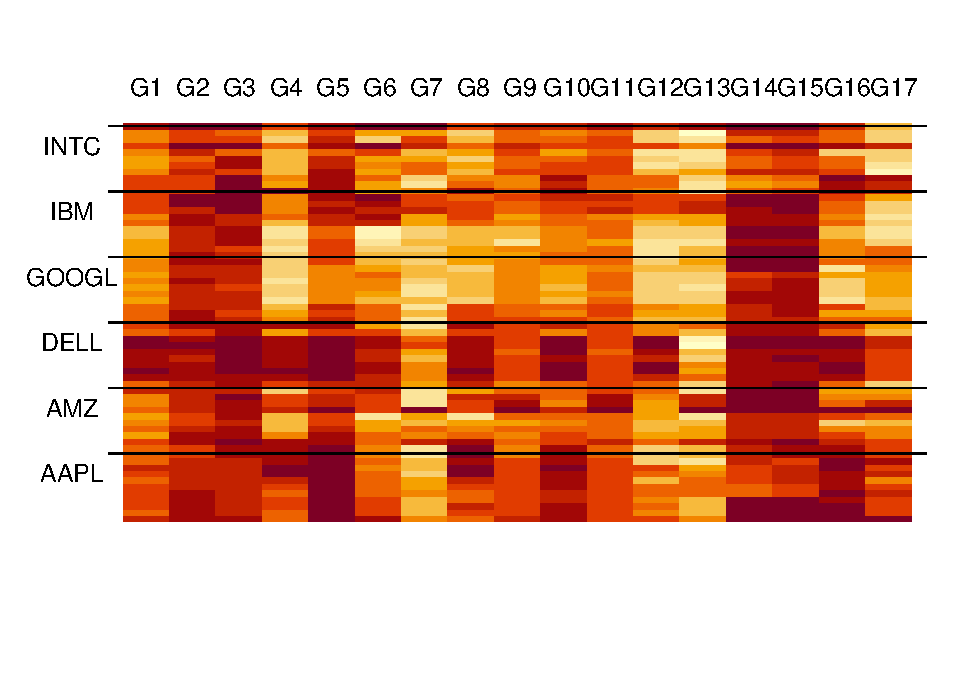
\includegraphics{20210219_sustain_dim_files/figure-latex/figeucl-1.pdf}
\caption{\label{fig:figeucl}Normalized minimum Euclidean distance based on the obtained report contexts embeddings over the available company-years (rows, starting with earlier years on the top) to the SDGs (columns). Lighter colors correspond to smaller distances.}
\end{figure}

In Figure \ref{fig:figeucl}, we use normalized minimum Euclidean distance to compare the reports contents with the SDGs. Thereby, we first compute the Euclidean distance between each context (report section) and the SDG texts and then take the minimum of the distance over all sections of a report as the resulting dissimilarity measure to a particular goal.

Using the average dissimilarity over the years, we construct a rating of the considered firms aith respect to each of the SDGs. The rating is presented in Table \ref{tab:tab01}.

\begin{table}

\caption{\label{tab:tab01}Company rating (from closest to farthest) with respect to the individual SDGs based on the average Euclidean distance of the report embeddings.}
\centering
\begin{tabular}[t]{l|l}
\hline
Goal & Rating\\
\hline
Goal\_1 & AAPL, AMZ, DELL, GOOGL, IBM, INTC, MSFT, SSU\\
\hline
Goal\_2 & INTC, AMZ, SSU, DELL, IBM, AAPL, MSFT, GOOGL\\
\hline
Goal\_3 & SSU, AMZ, DELL, INTC, AAPL, MSFT, IBM, GOOGL\\
\hline
Goal\_4 & SSU, INTC, IBM, AAPL, AMZ, DELL, MSFT, GOOGL\\
\hline
Goal\_5 & INTC, SSU, AMZ, IBM, MSFT, DELL, AAPL, GOOGL\\
\hline
Goal\_6 & INTC, AMZ, IBM, SSU, DELL, MSFT, AAPL, GOOGL\\
\hline
Goal\_7 & INTC, AMZ, SSU, IBM, AAPL, DELL, MSFT, GOOGL\\
\hline
Goal\_8 & IBM, INTC, AAPL, DELL, MSFT, GOOGL, AMZ, SSU\\
\hline
Goal\_9 & INTC, SSU, AMZ, MSFT, DELL, IBM, AAPL, GOOGL\\
\hline
Goal\_10 & INTC, AMZ, MSFT, IBM, SSU, GOOGL, AAPL, DELL\\
\hline
Goal\_11 & INTC, AMZ, SSU, DELL, IBM, MSFT, AAPL, GOOGL\\
\hline
Goal\_12 & INTC, MSFT, AMZ, AAPL, IBM, GOOGL, SSU, DELL\\
\hline
Goal\_13 & INTC, SSU, AMZ, IBM, AAPL, DELL, MSFT, GOOGL\\
\hline
Goal\_14 & INTC, GOOGL, SSU, AMZ, AAPL, IBM, MSFT, DELL\\
\hline
Goal\_15 & SSU, MSFT, AAPL, AMZ, IBM, INTC, GOOGL, DELL\\
\hline
Goal\_16 & SSU, MSFT, AMZ, AAPL, IBM, INTC, GOOGL, DELL\\
\hline
Goal\_17 & INTC, AMZ, DELL, IBM, SSU, MSFT, AAPL, GOOGL\\
\hline
\end{tabular}
\end{table}

\begin{figure}
\centering
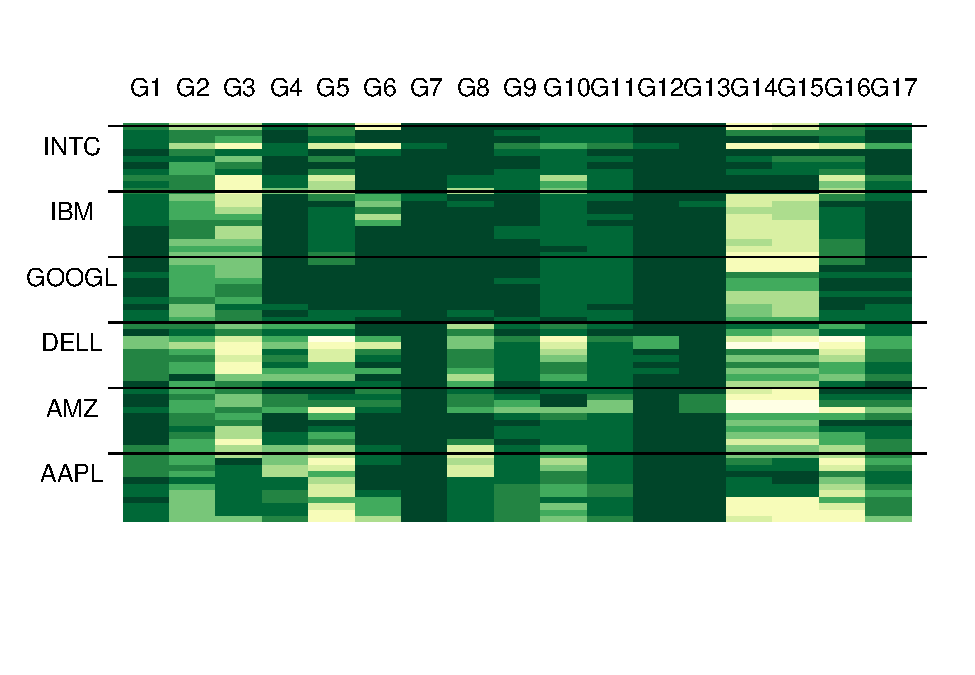
\includegraphics{20210219_sustain_dim_files/figure-latex/figcos-1.pdf}
\caption{\label{fig:figcos}Maximum cosine similarity based on the obtained report contexts embeddings over the available company-years (rows, starting with earlier years on the top) to the SDGs (columns). Darker colors correspond to higher similarity values.}
\end{figure}

In Figure \ref{fig:figcos}, we use cosine similarity of the report representations in the obtained latent topic space in order to compare the considered reports with the SDGs. Thereby, we first compute the cosine similarity between each context (report section) and the SDG texts and then take the maximum over all sections of a report as the resulting similarity measure.

By averaging the similarities for each company over the years, we construct a cosine similarity based rating of the considered firms with respect to each of the SDGs. The rating is presented in Table \ref{tab:tab02}.

\begin{table}

\caption{\label{tab:tab02}Company rating (from most similar to least similar) with respect to the individual SDGs based on the average cosine similarity of the report embeddings.}
\centering
\begin{tabular}[t]{l|l}
\hline
Goal & Rating\\
\hline
Goal\_1 & SSU, MSFT, INTC, IBM, GOOGL, DELL, AMZ, AAPL\\
\hline
Goal\_2 & INTC, AMZ, DELL, SSU, IBM, AAPL, MSFT, GOOGL\\
\hline
Goal\_3 & AMZ, MSFT, GOOGL, IBM, SSU, DELL, INTC, AAPL\\
\hline
Goal\_4 & AAPL, IBM, DELL, SSU, INTC, AMZ, MSFT, GOOGL\\
\hline
Goal\_5 & INTC, AMZ, SSU, MSFT, IBM, DELL, GOOGL, AAPL\\
\hline
Goal\_6 & INTC, IBM, AMZ, SSU, DELL, MSFT, GOOGL, AAPL\\
\hline
Goal\_7 & INTC, AMZ, IBM, AAPL, DELL, SSU, MSFT, GOOGL\\
\hline
Goal\_8 & AMZ, IBM, AAPL, GOOGL, INTC, DELL, MSFT, SSU\\
\hline
Goal\_9 & SSU, INTC, AMZ, MSFT, IBM, DELL, AAPL, GOOGL\\
\hline
Goal\_10 & INTC, IBM, AMZ, MSFT, SSU, GOOGL, AAPL, DELL\\
\hline
Goal\_11 & INTC, IBM, AMZ, SSU, DELL, MSFT, AAPL, GOOGL\\
\hline
Goal\_12 & IBM, INTC, MSFT, SSU, AMZ, GOOGL, AAPL, DELL\\
\hline
Goal\_13 & IBM, INTC, AMZ, AAPL, SSU, DELL, MSFT, GOOGL\\
\hline
Goal\_14 & AMZ, IBM, INTC, GOOGL, AAPL, SSU, MSFT, DELL\\
\hline
Goal\_15 & SSU, IBM, AAPL, MSFT, AMZ, GOOGL, INTC, DELL\\
\hline
Goal\_16 & SSU, AAPL, IBM, MSFT, AMZ, GOOGL, INTC, DELL\\
\hline
Goal\_17 & INTC, IBM, SSU, AMZ, DELL, MSFT, GOOGL, AAPL\\
\hline
\end{tabular}
\end{table}

Both ratings exhibit only minor differences, such that our methodology is fairly robust to the choice between the two (dis)similarity measures. (rating correlation?)

In our framework, we can also consider linear combinations of the goals based on individual preferences, such that an individual goal may be constructed for tailored sustainability assessment.

In order to considering individual preferences, we take a linear combination of the goals with weights \(\beta=(\beta_1,\ldots,\beta_{17})^\top\) then \(C\beta\approx UQ^\top\beta\) defines a ``personalized'' goal in terms of term occurrences approximated by the factorization. In Table \ref{tab:tab03}, we provide an example of such tailored sustainability assessment using four different combinations of SDGs, where all goals are equally weighted (``all\_equal''), only the goals, addressing basic human needs (SDGs 1-6) are equally weighted (``basic\_needs''), only the goals concerning society and infrastructure developement (SDGs 7-12 and 16-17) are equaly weighted (``fair\_society''), only the goals addressing climated, plat and animal life (SDGs 13-15) are equally weighted (``climate\_life''), and all other goals have zero weights.

\begin{table}

\caption{\label{tab:tab03}Company rating (from closest to farthest) with respect to the individual SDG combination based on the average Euclidean distance of the report embeddings in year 2022.}
\centering
\begin{tabular}[t]{l|l}
\hline
goal & rating\\
\hline
all\_equal & INTC, DELL, AMZ, IBM, MSFT, SSU, AAPL, GOOGL\\
\hline
basic\_needs & AMZ, INTC, DELL, IBM, AAPL, SSU, MSFT, GOOGL\\
\hline
fair\_society & DELL, INTC, AMZ, MSFT, IBM, AAPL, SSU, GOOGL\\
\hline
climate\_life & MSFT, IBM, AMZ, INTC, AAPL, DELL, GOOGL, SSU\\
\hline
\end{tabular}
\end{table}

As shown, the ratings can be quite different depending on the concrete preferences. Thereby, any linear combination of the goals can build a basis for such a comparison. This makes the procedure very flexible. moreover, any user defined (dis)similarity metric can be applied to the resulting embeddings in the topic space, which grant additional flexibility.

\hypertarget{conclusion}{%
\section{Conclusion}\label{conclusion}}

We proposed a non-negative matrix co-factorization for topic extraction with side information, which results in a low dimensional representation in a prestructured topic space. The method is simple to implement and does not require any manual preprocessing as other comparable methods. It delivers transparent and interpretable results with many use cases. The resulting contextual embeddings in a low dimensional topic space are used to compare the sustainablility related reports of chosen listed tech firms via two dissimilarity measures: Euclidean distance and cosine similarity. The results show, that our procedure can efficiently assists financial decisions under tailored SDGs based preferences.
Nevertheless, we can not oversee some important limitations as the assumption that the reports texts contain coincide information on firms' sustainability actions.

\hypertarget{references}{%
\section*{References}\label{references}}
\addcontentsline{toc}{section}{References}

\hypertarget{refs}{}
\begin{CSLReferences}{1}{0}
\leavevmode\vadjust pre{\hypertarget{ref-quanteda}{}}%
Benoit, Kenneth, Kohei Watanabe, Haiyan Wang, Paul Nulty, Adam Obeng, Stefan Müller, and Akitaka Matsuo. 2018. {``Quanteda: An r Package for the Quantitative Analysis of Textual Data.''} \emph{Journal of Open Source Software} 3 (30): 774. \url{https://doi.org/10.21105/joss.00774}.

\leavevmode\vadjust pre{\hypertarget{ref-berg2022}{}}%
Berg, Florian, Julian F Kölbel, and Roberto Rigobon. 2022. {``{Aggregate Confusion: The Divergence of ESG Ratings*}.''} \emph{Review of Finance} 26 (6): 1315--44. \url{https://doi.org/10.1093/rof/rfac033}.

\leavevmode\vadjust pre{\hypertarget{ref-blei2003}{}}%
Blei, David M., Andrew Y. Ng, and Michael I. Jordan. 2003. {``Latent Dirichlet Allocation.''} \emph{J. Mach. Learn. Res.} 3 (null): 993--1022.

\leavevmode\vadjust pre{\hypertarget{ref-chen2023}{}}%
Chen, Weisi, Fethi Rabhi, Wenqi Liao, and Islam Al-Qudah. 2023. {``Leveraging State-of-the-Art Topic Modeling for News Impact Analysis on Financial Markets: A Comparative Study.''} \emph{Electronics} 12 (12). \url{https://doi.org/10.3390/electronics12122605}.

\leavevmode\vadjust pre{\hypertarget{ref-CHEN2019}{}}%
Chen, Yong, Hui Zhang, Rui Liu, Zhiwen Ye, and Jianying Lin. 2019. {``Experimental Explorations on Short Text Topic Mining Between LDA and NMF Based Schemes.''} \emph{Knowledge-Based Systems} 163: 1--13. https://doi.org/\url{https://doi.org/10.1016/j.knosys.2018.08.011}.

\leavevmode\vadjust pre{\hypertarget{ref-chen2017}{}}%
Chen, Yu, Rhaad M. Rabbani, Aparna Gupta, and Mohammed J. Zaki. 2017. {``Comparative Text Analytics via Topic Modeling in Banking.''} In \emph{2017 IEEE Symposium Series on Computational Intelligence (SSCI)}, 1--8. \url{https://doi.org/10.1109/SSCI.2017.8280945}.

\leavevmode\vadjust pre{\hypertarget{ref-churchill2022}{}}%
Churchill, Rob, and Lisa Singh. 2022. {``The Evolution of Topic Modeling.''} \emph{ACM Comput. Surv.} 54 (10s). \url{https://doi.org/10.1145/3507900}.

\leavevmode\vadjust pre{\hypertarget{ref-cichocki2007}{}}%
Cichocki, Andrzej, Rafal Zdunek, and Shun-ichi Amari. 2007. {``Hierarchical ALS Algorithms for Nonnegative Matrix and 3D Tensor Factorization.''} In \emph{Independent Component Analysis and Signal Separation}, edited by Mike E. Davies, Christopher J. James, Samer A. Abdallah, and Mark D. Plumbley, 169--76. Berlin, Heidelberg: Springer Berlin Heidelberg.

\leavevmode\vadjust pre{\hypertarget{ref-deerwester1990}{}}%
Deerwester, Scott, Susan T. Dumais, George W. Furnas, Thomas K. Landauer, and Richard Harshman. 1990. {``Indexing by Latent Semantic Analysis.''} \emph{Journal of the American Society for Information Science} 41 (6): 391--407. https://doi.org/\url{https://doi.org/10.1002/(SICI)1097-4571(199009)41:6\%3C391::AID-ASI1\%3E3.0.CO;2-9}.

\leavevmode\vadjust pre{\hypertarget{ref-degleris2019}{}}%
Degleris, Anthony, Ben Antin, Surya Ganguli, and Alex H Williams. 2019. {``Fast Convolutive Nonnegative Matrix Factorization Through Coordinate and Block Coordinate Updates.''} \url{https://arxiv.org/abs/1907.00139}.

\leavevmode\vadjust pre{\hypertarget{ref-egger2022}{}}%
Egger, Roman, and Joanne Yu. 2022. {``A Topic Modeling Comparison Between LDA, NMF, Top2Vec, and BERTopic to Demystify Twitter Posts.''} \emph{Frontiers in Sociology} 7. \url{https://doi.org/10.3389/fsoc.2022.886498}.

\leavevmode\vadjust pre{\hypertarget{ref-eshima2023}{}}%
Eshima, Shusei, Kosuke Imai, and Tomoya Sasaki. 2023. {``Keyword Assisted Topic Models.''} \url{https://arxiv.org/abs/2004.05964}.

\leavevmode\vadjust pre{\hypertarget{ref-fang2011}{}}%
Fang, Yi, and Luo Si. 2011. {``Matrix Co-Factorization for Recommendation with Rich Side Information and Implicit Feedback.''} In \emph{Proceedings of the 2nd International Workshop on Information Heterogeneity and Fusion in Recommender Systems}, 65--69. HetRec '11. New York, NY, USA: Association for Computing Machinery. \url{https://doi.org/10.1145/2039320.2039330}.

\leavevmode\vadjust pre{\hypertarget{ref-figuera2024}{}}%
Figuera, Pau, and Pablo García Bringas. 2024. {``Revisiting Probabilistic Latent Semantic Analysis: Extensions, Challenges and Insights.''} \emph{Technologies} 12 (1). \url{https://doi.org/10.3390/technologies12010005}.

\leavevmode\vadjust pre{\hypertarget{ref-gupta2020}{}}%
Gupta, Aaryan, Vinya Dengre, Hamza Abubakar Kheruwala, and Manan Shah. 2020. {``Comprehensive Review of Text-Mining Applications in Finance.''} \emph{Financial Innovation} 6 (1): 1--25. \url{https://doi.org/10.1186/s40854-020-00205-1}.

\leavevmode\vadjust pre{\hypertarget{ref-Harandizadeh2022}{}}%
Harandizadeh, Bahareh, J. Hunter Priniski, and Fred Morstatter. 2022. {``Keyword Assisted Embedded Topic Model.''} In \emph{Proceedings of the Fifteenth {ACM} International Conference on Web Search and Data Mining}. {ACM}. \url{https://doi.org/10.1145/3488560.3498518}.

\leavevmode\vadjust pre{\hypertarget{ref-hofmann1999}{}}%
Hofmann, Thomas. 1999. {``Probabilistic Latent Semantic Indexing.''} In \emph{Proceedings of the 22nd Annual International ACM SIGIR Conference on Research and Development in Information Retrieval}, 50--57. SIGIR '99. New York, NY, USA: Association for Computing Machinery. \url{https://doi.org/10.1145/312624.312649}.

\leavevmode\vadjust pre{\hypertarget{ref-kang2022}{}}%
Kang, Hyewon, and Jinho Kim. 2022. {``Analyzing and Visualizing Text Information in Corporate Sustainability Reports Using Natural Language Processing Methods.''} \emph{Applied Sciences} 12 (11). \url{https://doi.org/10.3390/app12115614}.

\leavevmode\vadjust pre{\hypertarget{ref-lee2000}{}}%
Lee, Daniel, and H. Sebastian Seung. 2000. {``Algorithms for Non-Negative Matrix Factorization.''} In \emph{Advances in Neural Information Processing Systems}, edited by T. Leen, T. Dietterich, and V. Tresp. Vol. 13. MIT Press. \url{https://proceedings.neurips.cc/paper_files/paper/2000/file/f9d1152547c0bde01830b7e8bd60024c-Paper.pdf}.

\leavevmode\vadjust pre{\hypertarget{ref-LI2017}{}}%
Li, Guowen, Xiaoqian Zhu, Jun Wang, Dengsheng Wu, and Jianping Li. 2017. {``Using LDA Model to Quantify and Visualize Textual Financial Stability Report.''} \emph{Procedia Computer Science} 122: 370--76. https://doi.org/\url{https://doi.org/10.1016/j.procs.2017.11.382}.

\leavevmode\vadjust pre{\hypertarget{ref-loughran2016}{}}%
LOUGHRAN, TIM, and BILL MCDONALD. 2016. {``Textual Analysis in Accounting and Finance: A Survey.''} \emph{Journal of Accounting Research} 54 (4): 1187--1230. https://doi.org/\url{https://doi.org/10.1111/1475-679X.12123}.

\leavevmode\vadjust pre{\hypertarget{ref-luo2019}{}}%
Luo, Ling, Haoran Xie, Yanghui Rao, and Fu Lee Wang. 2019. {``Personalized Recommendation by Matrix Co-Factorization with Tags and Time Information.''} \emph{Expert Systems with Applications} 119: 311--21. https://doi.org/\url{https://doi.org/10.1016/j.eswa.2018.11.003}.

\leavevmode\vadjust pre{\hypertarget{ref-NUGUMANOVA2022}{}}%
Nugumanova, Aliya, Darkhan Akhmed-Zaki, Madina Mansurova, Yerzhan Baiburin, and Almasbek Maulit. 2022. {``NMF-Based Approach to Automatic Term Extraction.''} \emph{Expert Systems with Applications} 199: 117179. https://doi.org/\url{https://doi.org/10.1016/j.eswa.2022.117179}.

\leavevmode\vadjust pre{\hypertarget{ref-rr}{}}%
R Core Team. 2023. \emph{R: A Language and Environment for Statistical Computing}. Vienna, Austria: R Foundation for Statistical Computing. \url{https://www.R-project.org/}.

\leavevmode\vadjust pre{\hypertarget{ref-rao2015}{}}%
Rao, Nikhil, Hsiang-Fu Yu, Pradeep K Ravikumar, and Inderjit S Dhillon. 2015. {``Collaborative Filtering with Graph Information: Consistency and Scalable Methods.''} In \emph{Advances in Neural Information Processing Systems}, edited by C. Cortes, N. Lawrence, D. Lee, M. Sugiyama, and R. Garnett. Vol. 28. Curran Associates, Inc. \url{https://proceedings.neurips.cc/paper_files/paper/2015/file/f4573fc71c731d5c362f0d7860945b88-Paper.pdf}.

\leavevmode\vadjust pre{\hypertarget{ref-text2vec}{}}%
Selivanov, Dmitriy, Manuel Bickel, and Qing Wang. 2022. \emph{Text2vec: Modern Text Mining Framework for r}. \url{https://CRAN.R-project.org/package=text2vec}.

\leavevmode\vadjust pre{\hypertarget{ref-SULEMAN2021}{}}%
Suleman, Raja Muhammad, and Ioannis Korkontzelos. 2021. {``Extending Latent Semantic Analysis to Manage Its Syntactic Blindness.''} \emph{Expert Systems with Applications} 165: 114130. https://doi.org/\url{https://doi.org/10.1016/j.eswa.2020.114130}.

\leavevmode\vadjust pre{\hypertarget{ref-thompson-mimno-2018}{}}%
Thompson, Laure, and David Mimno. 2018. {``Authorless Topic Models: Biasing Models Away from Known Structure.''} In \emph{Proceedings of the 27th International Conference on Computational Linguistics}, edited by Emily M. Bender, Leon Derczynski, and Pierre Isabelle, 3903--14. Santa Fe, New Mexico, USA: Association for Computational Linguistics. \url{https://aclanthology.org/C18-1329}.

\leavevmode\vadjust pre{\hypertarget{ref-vangara2020}{}}%
Vangara, Raviteja, Erik Skau, Gopinath Chennupati, Hristo Djidjev, Thomas Tierney, James P. Smith, Manish Bhattarai, Valentin G. Stanev, and Boian S. Alexandrov. 2020. {``Semantic Nonnegative Matrix Factorization with Automatic Model Determination for Topic Modeling.''} In \emph{2020 19th IEEE International Conference on Machine Learning and Applications (ICMLA)}, 328--35. \url{https://doi.org/10.1109/ICMLA51294.2020.00060}.

\leavevmode\vadjust pre{\hypertarget{ref-watanabe2022}{}}%
Watanabe, Kohei, and Yuan Zhou. 2022. {``Theory-Driven Analysis of Large Corpora: Semisupervised Topic Classification of the UN Speeches.''} \emph{Social Science Computer Review} 40 (2): 346--66. \url{https://doi.org/10.1177/0894439320907027}.

\leavevmode\vadjust pre{\hypertarget{ref-Yang2015}{}}%
Yang, Qingquan, and Weijiang Li. 2015/07. {``The LDA Topic Model Extension Study.''} In \emph{Proceedings of the International Conference on Logistics, Engineering, Management and Computer Science}, 857--60. Atlantis Press. \url{https://doi.org/10.2991/lemcs-15.2015.169}.

\leavevmode\vadjust pre{\hypertarget{ref-zahng2020_graph}{}}%
Zhang, Yupei, Yue Yun, Huan Dai, Jiaqi Cui, and Xuequn Shang. 2020. {``Graphs Regularized Robust Matrix Factorization and Its Application on Student Grade Prediction.''} \emph{Applied Sciences} 10 (5). \url{https://doi.org/10.3390/app10051755}.

\leavevmode\vadjust pre{\hypertarget{ref-Zhao2021}{}}%
Zhao, He, Dinh Q. Phung, Viet Huynh, Yuan Jin, Lan Du, and Wray L. Buntine. 2021. {``Topic Modelling Meets Deep Neural Networks: A Survey.''} In \emph{International Joint Conference on Artificial Intelligence}. \url{https://api.semanticscholar.org/CorpusID:232076325}.

\end{CSLReferences}

\end{document}
